\documentclass[12 pt, a4paper]{article}

\usepackage[T1]{fontenc}
\usepackage[polish]{babel}
\usepackage[utf8]{inputenc}
\usepackage{graphicx, amssymb, amsmath, enumerate, multicol}

\author {Konrad Pagacz}

\begin{document}
\begin{enumerate}

\item Proszę utworzyć następującą tabelę

	\begin{tabular} { | c | c | c |} \hline \hline
	\textbf{Lp.}	&	\textbf{Miasto}	&	\textbf{Państwo}	\\ \hline
	1.	&	Warszawa	&	Polska \\ \hline
	2.	&	Praga	&	Czechy	\\ \hline
	3.	&	Barcelona	&	Hiszpania	\\ \hline
	4.	&	Berlin	&	Niemcy	\\ \hline
	5.	&	Wiedeń	&	Austria	\\ \hline
	6.	&	Zakopane	&	Polska	\\ 
		\hline \hline
	\end{tabular}

\item Proszę utworzyć tabelę, w której będą umieszczone wartości logiczne koniunkcji, alternatywy, implikacji i równoważności

		\begin{tabular} {| c | c | c | c | c | c |} \hline
		$p$	&	$q$	&	$p \wedge q$	&	$p \vee q$	&	$p \Rightarrow q$	&	$p \Leftrightarrow q$ \\ \hline
		0	&	0	&	0	&	0	&	1	&	1	\\ \hline
		0	&	1	&	0	&	1	&	1	&	0	\\ \hline
		1	&	0	&	0	&	1	&	0	&	0	\\ \hline
		1	&	1	&	1	&	1	&	1	&	1	\\ \hline
		\end{tabular}
		
\item Proszę utworzyć następującą tabelę:

	\begin{tabular}	{| p{2.5cm} | p{8cm} |} \hline
	Znak zodiaku	&	Charakterystyka	\\	\hline
	Wodnik	&	Wodniki nie lubią utartych schematów i usta-lonych reguł. Zamiast tkwić w tym, co sprawdzone, wybiegają myślą w przyszłość. 	Przeważnie sa tolerancyjne i niewiele rzeczy jest w stanie je zdziwić. \\ \hline
	Rak	&	Raki mogą sprawiać wrażenie bojaźliwych i nieśmiałych. Czasem wręcz zachowują się tak, jakby cały świat stanowił dla nich zagrożenie. Bardzo silnie się przywiązują, zarównodo ludzi, jak i do rzeczy. \\ \hline
	Byk	&	Byki poświęcają dużo uwagi przyjemnościom zmysłowym i wygodom. Można powiedzieć,że odbierając rzeczywistość wszystkimi zmysłami najbardziej czują, że żyją. Są niezwykle stałe i konsekwentne w swoich upodobaniachi zapatrywaniach. \\ \hline
	\end{tabular}

\pagebreak	
\item Proszę utworzyć następującą tabelę:

	{\centering
	\begin{tabular} {| c | r | r |} \hline
	$x$	&	\multicolumn{2}{| c |}{$x^n$} \\ \cline{2-3}
		&	$n = 2$	&	$n=3$	\\ \hline
	$1$	&	$1$	&	$1$	\\ \hline
	$2$	&	$4$	&	$8$	\\ \hline
	$3$	&	$9$	&	$27$	\\ \hline
	$4$	&	$16$	&	$64$	\\ \hline
	\end{tabular}
	\par}
	
\item Złożyć następujący tekst z grafiką (z pliku jpg)

	\begin{center}
	\textbf{FIRMA zaprasza wszystkich chętnych na kursy \LaTeX-a}
	\end{center}
	\centering 
\includegraphics[height=2cm, width=3cm]{logo.jpg}
	\begin{center}
	\textbf{Zapewniamy}
	\begin{itemize}
		\begin{multicols}{2}
			\item[$\star$] doświadczoną kadrę
			\item[$\star$] dogodne terminy spotkań
			\item[$\star$] atrakcyjne ceny
			\item[$\star$] miłą atmosferę podcza pracy
		\end{multicols}
	\end{itemize}
	\end{center}

\item Utworzyć tabelę (bez obramowania) z elementami grafiki:
    \begin{tabular}{p{2.5cm} p{8cm}}
    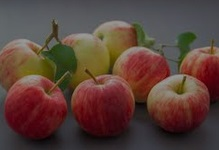
\includegraphics[height=2cm, width=2cm]{jablka.jpg}  &   pyszne jabłka \\
    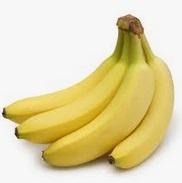
\includegraphics[height=2cm, width=2cm]{banany.jpg} &   odżywcze banany \\
    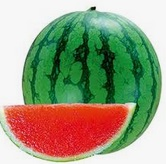
\includegraphics[height=2cm, width=2cm]{arbuz.jpg}  &   soczysty arbuz \\
    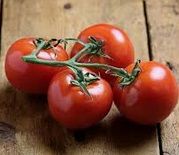
\includegraphics[height=2cm, width=2cm]{pomidory.jpg}   &   wspaniałe pomidory
    \end{tabular}

\end{enumerate}
\end{document}
